\documentclass[]{article}
\usepackage{lmodern}
\usepackage{amssymb,amsmath}
\usepackage{ifxetex,ifluatex}
\usepackage{fixltx2e} % provides \textsubscript
\ifnum 0\ifxetex 1\fi\ifluatex 1\fi=0 % if pdftex
  \usepackage[T1]{fontenc}
  \usepackage[utf8]{inputenc}
\else % if luatex or xelatex
  \ifxetex
    \usepackage{mathspec}
  \else
    \usepackage{fontspec}
  \fi
  \defaultfontfeatures{Ligatures=TeX,Scale=MatchLowercase}
\fi
% use upquote if available, for straight quotes in verbatim environments
\IfFileExists{upquote.sty}{\usepackage{upquote}}{}
% use microtype if available
\IfFileExists{microtype.sty}{%
\usepackage{microtype}
\UseMicrotypeSet[protrusion]{basicmath} % disable protrusion for tt fonts
}{}
\usepackage[margin=1in]{geometry}
\usepackage{hyperref}
\hypersetup{unicode=true,
            pdftitle={An attempt at analyzing the TCEC Season 15 SuFi openings},
            pdfauthor={Joseph V. Iris},
            pdfborder={0 0 0},
            breaklinks=true}
\urlstyle{same}  % don't use monospace font for urls
\usepackage{color}
\usepackage{fancyvrb}
\newcommand{\VerbBar}{|}
\newcommand{\VERB}{\Verb[commandchars=\\\{\}]}
\DefineVerbatimEnvironment{Highlighting}{Verbatim}{commandchars=\\\{\}}
% Add ',fontsize=\small' for more characters per line
\usepackage{framed}
\definecolor{shadecolor}{RGB}{248,248,248}
\newenvironment{Shaded}{\begin{snugshade}}{\end{snugshade}}
\newcommand{\AlertTok}[1]{\textcolor[rgb]{0.94,0.16,0.16}{#1}}
\newcommand{\AnnotationTok}[1]{\textcolor[rgb]{0.56,0.35,0.01}{\textbf{\textit{#1}}}}
\newcommand{\AttributeTok}[1]{\textcolor[rgb]{0.77,0.63,0.00}{#1}}
\newcommand{\BaseNTok}[1]{\textcolor[rgb]{0.00,0.00,0.81}{#1}}
\newcommand{\BuiltInTok}[1]{#1}
\newcommand{\CharTok}[1]{\textcolor[rgb]{0.31,0.60,0.02}{#1}}
\newcommand{\CommentTok}[1]{\textcolor[rgb]{0.56,0.35,0.01}{\textit{#1}}}
\newcommand{\CommentVarTok}[1]{\textcolor[rgb]{0.56,0.35,0.01}{\textbf{\textit{#1}}}}
\newcommand{\ConstantTok}[1]{\textcolor[rgb]{0.00,0.00,0.00}{#1}}
\newcommand{\ControlFlowTok}[1]{\textcolor[rgb]{0.13,0.29,0.53}{\textbf{#1}}}
\newcommand{\DataTypeTok}[1]{\textcolor[rgb]{0.13,0.29,0.53}{#1}}
\newcommand{\DecValTok}[1]{\textcolor[rgb]{0.00,0.00,0.81}{#1}}
\newcommand{\DocumentationTok}[1]{\textcolor[rgb]{0.56,0.35,0.01}{\textbf{\textit{#1}}}}
\newcommand{\ErrorTok}[1]{\textcolor[rgb]{0.64,0.00,0.00}{\textbf{#1}}}
\newcommand{\ExtensionTok}[1]{#1}
\newcommand{\FloatTok}[1]{\textcolor[rgb]{0.00,0.00,0.81}{#1}}
\newcommand{\FunctionTok}[1]{\textcolor[rgb]{0.00,0.00,0.00}{#1}}
\newcommand{\ImportTok}[1]{#1}
\newcommand{\InformationTok}[1]{\textcolor[rgb]{0.56,0.35,0.01}{\textbf{\textit{#1}}}}
\newcommand{\KeywordTok}[1]{\textcolor[rgb]{0.13,0.29,0.53}{\textbf{#1}}}
\newcommand{\NormalTok}[1]{#1}
\newcommand{\OperatorTok}[1]{\textcolor[rgb]{0.81,0.36,0.00}{\textbf{#1}}}
\newcommand{\OtherTok}[1]{\textcolor[rgb]{0.56,0.35,0.01}{#1}}
\newcommand{\PreprocessorTok}[1]{\textcolor[rgb]{0.56,0.35,0.01}{\textit{#1}}}
\newcommand{\RegionMarkerTok}[1]{#1}
\newcommand{\SpecialCharTok}[1]{\textcolor[rgb]{0.00,0.00,0.00}{#1}}
\newcommand{\SpecialStringTok}[1]{\textcolor[rgb]{0.31,0.60,0.02}{#1}}
\newcommand{\StringTok}[1]{\textcolor[rgb]{0.31,0.60,0.02}{#1}}
\newcommand{\VariableTok}[1]{\textcolor[rgb]{0.00,0.00,0.00}{#1}}
\newcommand{\VerbatimStringTok}[1]{\textcolor[rgb]{0.31,0.60,0.02}{#1}}
\newcommand{\WarningTok}[1]{\textcolor[rgb]{0.56,0.35,0.01}{\textbf{\textit{#1}}}}
\usepackage{graphicx,grffile}
\makeatletter
\def\maxwidth{\ifdim\Gin@nat@width>\linewidth\linewidth\else\Gin@nat@width\fi}
\def\maxheight{\ifdim\Gin@nat@height>\textheight\textheight\else\Gin@nat@height\fi}
\makeatother
% Scale images if necessary, so that they will not overflow the page
% margins by default, and it is still possible to overwrite the defaults
% using explicit options in \includegraphics[width, height, ...]{}
\setkeys{Gin}{width=\maxwidth,height=\maxheight,keepaspectratio}
\IfFileExists{parskip.sty}{%
\usepackage{parskip}
}{% else
\setlength{\parindent}{0pt}
\setlength{\parskip}{6pt plus 2pt minus 1pt}
}
\setlength{\emergencystretch}{3em}  % prevent overfull lines
\providecommand{\tightlist}{%
  \setlength{\itemsep}{0pt}\setlength{\parskip}{0pt}}
\setcounter{secnumdepth}{0}
% Redefines (sub)paragraphs to behave more like sections
\ifx\paragraph\undefined\else
\let\oldparagraph\paragraph
\renewcommand{\paragraph}[1]{\oldparagraph{#1}\mbox{}}
\fi
\ifx\subparagraph\undefined\else
\let\oldsubparagraph\subparagraph
\renewcommand{\subparagraph}[1]{\oldsubparagraph{#1}\mbox{}}
\fi

%%% Use protect on footnotes to avoid problems with footnotes in titles
\let\rmarkdownfootnote\footnote%
\def\footnote{\protect\rmarkdownfootnote}

%%% Change title format to be more compact
\usepackage{titling}

% Create subtitle command for use in maketitle
\providecommand{\subtitle}[1]{
  \posttitle{
    \begin{center}\large#1\end{center}
    }
}

\setlength{\droptitle}{-2em}

  \title{An attempt at analyzing the TCEC Season 15 SuFi openings}
    \pretitle{\vspace{\droptitle}\centering\huge}
  \posttitle{\par}
    \author{Joseph V. Iris}
    \preauthor{\centering\large\emph}
  \postauthor{\par}
      \predate{\centering\large\emph}
  \postdate{\par}
    \date{2019-05-28}


\begin{document}
\maketitle

My aim here is to try to analyze and make sense of what happened in the
TCEC Seasono 15 SuFi, based on the ECO group of openings. Based on
Jeroen Noomen's
\href{http://blogchess2016.blogspot.com/2019/04/opening-selection-tcec-15-superfinal.html}{blog},
the following are the intended openings:

\begin{verbatim}
ECO code distribution
ECO A: 15 lines
ECO B: 14 lines
ECO C: 11 lines
ECO D: 3 lines
ECO E: 7 lines
\end{verbatim}

However, the ECO code distribution may have changed because of some
transpositions. I have stored the results of the TCEC Season 15 SuFi
\href{https://raw.githubusercontent.com/josephviruses/josephviruses.github.io/master/content/post/leelasf2.csv}{here}.

\begin{Shaded}
\begin{Highlighting}[]
\KeywordTok{library}\NormalTok{(tidyverse)}
\KeywordTok{library}\NormalTok{(elo)}
\KeywordTok{library}\NormalTok{(flextable)}
\KeywordTok{library}\NormalTok{(officer)}
\NormalTok{data <-}\StringTok{ }\KeywordTok{read_delim}\NormalTok{(}\StringTok{"./leelasf2.csv"}\NormalTok{, }\DataTypeTok{delim =} \StringTok{";"}\NormalTok{)}
\NormalTok{data }\OperatorTok\StringTok{ }\KeywordTok{flextable}\NormalTok{() }\OperatorTok\StringTok{ }\KeywordTok{autofit}\NormalTok{()}
\end{Highlighting}
\end{Shaded}

\includegraphics[width=8.35in,height=28.94in,keepaspectratio]{2018-05-28_elo_compute_files/figure-latex/unnamed-chunk-1-1.png}

First, let's estimate the ELO differences between Leela and Stockfish
after every game. Initially, the estimated ELO's are 3589 for Leela and
3587 for Stockfish.

Let \(R_A\) be the ELO of engine \(A\) and \(R_B\) be the rating of
engine \(B\). Then the expected result for engine A against B is given
by the logistic equation:

\begin{equation}
E_A = \frac{1}{1+10^{(R_A-R_B)/400}}.
\end{equation}

Solving this equation for \(R_A-R_B\), we have:

\begin{equation}
elodiff = R_A-R_B = 400\log_{10}\left( \frac{1-E_A}{E_A}\right)
\end{equation}

Here we note that \((1-E_A)/E_A\) can be expressed as win ratio / loss
ratio without loss of generality. That is, we can put the win ratio of
the leading engine in the numerator and we get the same result. The win
ratio is the sum of the wins and draws.

In R, there is a package called
\href{https://CRAN.R-project.org/package=elo}{\texttt{elo}} which we
will also use here. But we can write our own functions for this purpose.

\begin{Shaded}
\begin{Highlighting}[]
\NormalTok{elo <-}\StringTok{ }\ControlFlowTok{function}\NormalTok{(win_ratio) \{}\DecValTok{400} \OperatorTok{*}\StringTok{ }\KeywordTok{log10}\NormalTok{(win_ratio }\OperatorTok{/}\StringTok{ }\NormalTok{(}\DecValTok{1}\OperatorTok{-}\NormalTok{win_ratio))\}}
\end{Highlighting}
\end{Shaded}

We can also check for the standard errors of ELO differences using a
normal approximation.

\begin{Shaded}
\begin{Highlighting}[]
\NormalTok{denom95 <-}\StringTok{ }\ControlFlowTok{function}\NormalTok{(win_ratio, total) }\KeywordTok{qnorm}\NormalTok{(}\FloatTok{0.975}\NormalTok{) }\OperatorTok{*}\StringTok{ }\KeywordTok{sqrt}\NormalTok{(win_ratio }\OperatorTok{*}\StringTok{ }\NormalTok{(}\DecValTok{1}\OperatorTok{-}\NormalTok{win_ratio)}\OperatorTok{/}\NormalTok{(total}\DecValTok{-1}\NormalTok{))}
\end{Highlighting}
\end{Shaded}

We can also compute for the LOS as described in the
\href{https://www.chessprogramming.org/Match_Statistics}{chessprogramming
wiki site}. I used three estimators here. \texttt{LOS3} might become
untenable with large data sets, but we only have 100 rows of data here
so it will be fine.

\begin{Shaded}
\begin{Highlighting}[]
\NormalTok{LOS <-}\StringTok{ }\ControlFlowTok{function}\NormalTok{(wins_losses, total) }\KeywordTok{pnorm}\NormalTok{(total}\OperatorTok{/}\DecValTok{2}\NormalTok{, }\DataTypeTok{sd =}\NormalTok{ wins_losses)}
\NormalTok{LOS2 <-}\StringTok{ }\ControlFlowTok{function}\NormalTok{(wins, losses) }\KeywordTok{pnorm}\NormalTok{((wins}\OperatorTok{-}\NormalTok{losses)}\OperatorTok{/}\KeywordTok{sqrt}\NormalTok{(wins}\OperatorTok{+}\NormalTok{losses))}
\NormalTok{LOS3 <-}\StringTok{ }\ControlFlowTok{function}\NormalTok{(wins, losses, draws) \{}
\NormalTok{  total =}\StringTok{ }\NormalTok{wins }\OperatorTok{+}\StringTok{ }\NormalTok{losses }\OperatorTok{+}\StringTok{ }\NormalTok{draws}
\NormalTok{  exp =}\StringTok{ }\NormalTok{(wins}\OperatorTok{/}\NormalTok{total)}\OperatorTok{^}\NormalTok{wins }\OperatorTok{*}\StringTok{ }\NormalTok{(losses}\OperatorTok{/}\NormalTok{total)}\OperatorTok{^}\NormalTok{losses }\OperatorTok{*}\StringTok{ }\NormalTok{(draws}\OperatorTok{/}\NormalTok{total)}\OperatorTok{^}\NormalTok{draws}
\NormalTok{  factorials =}\StringTok{ }\KeywordTok{factorial}\NormalTok{(total)}\OperatorTok{/}\NormalTok{(}\KeywordTok{factorial}\NormalTok{(wins)}\OperatorTok{*}\KeywordTok{factorial}\NormalTok{(losses)}\OperatorTok{*}\KeywordTok{factorial}\NormalTok{(draws))}
\NormalTok{  P =}\StringTok{ }\NormalTok{factorials }\OperatorTok{*}\StringTok{ }\NormalTok{exp}
  \DecValTok{1}\OperatorTok{-}\NormalTok{P}
\NormalTok{\}}
\end{Highlighting}
\end{Shaded}

We will now extract the initials of the ECO codes, determin the points
of Leela and SF after each game, the win rate (by the leading engine)
after each game, the estimated ELO difference (\texttt{elodiff}) after
each game, and the three LOS estimates after each game.

\begin{Shaded}
\begin{Highlighting}[]
\NormalTok{data <-}\StringTok{ }\NormalTok{data }\OperatorTok
\StringTok{  }\KeywordTok{mutate}\NormalTok{(}\DataTypeTok{ECO2 =} \KeywordTok{substr}\NormalTok{(ECO1, }\DataTypeTok{start =} \DecValTok{1}\NormalTok{, }\DataTypeTok{stop =} \DecValTok{1}\NormalTok{)) }\OperatorTok
\StringTok{  }\CommentTok{# calculate Leela's scores}
\StringTok{  }\KeywordTok{mutate}\NormalTok{(}\DataTypeTok{points.Leela =}\NormalTok{ (White }\OperatorTok{==}\StringTok{ "Leela"}\NormalTok{) }\OperatorTok{*}\StringTok{ }\NormalTok{points.White }\OperatorTok{+}\StringTok{ }\NormalTok{(Black }\OperatorTok{==}\StringTok{ "Leela"}\NormalTok{) }\OperatorTok{*}\StringTok{ }\NormalTok{points.Black) }\OperatorTok
\StringTok{  }\CommentTok{# calculate SF's scores}
\StringTok{  }\KeywordTok{mutate}\NormalTok{(}\DataTypeTok{points.SF =}\NormalTok{ (White }\OperatorTok{==}\StringTok{ "SF"}\NormalTok{) }\OperatorTok{*}\StringTok{ }\NormalTok{points.White }\OperatorTok{+}\StringTok{ }\NormalTok{(Black }\OperatorTok{==}\StringTok{ "SF"}\NormalTok{) }\OperatorTok{*}\StringTok{ }\NormalTok{points.Black) }\OperatorTok
\StringTok{  }\KeywordTok{mutate}\NormalTok{(}\DataTypeTok{results.Leela =} \KeywordTok{case_when}\NormalTok{(points.Leela }\OperatorTok{==}\StringTok{ }\DecValTok{1}\OperatorTok{~}\StringTok{"Win"}\NormalTok{, }
\NormalTok{                                   points.Leela }\OperatorTok{==}\StringTok{ }\FloatTok{0.5}\OperatorTok{~}\StringTok{"Draw"}\NormalTok{,}
\NormalTok{                                   points.Leela }\OperatorTok{==}\StringTok{ }\DecValTok{0}\OperatorTok{~}\StringTok{"Loss"}\NormalTok{)) }\OperatorTok
\StringTok{  }\KeywordTok{mutate}\NormalTok{(}\DataTypeTok{results.SF =} \KeywordTok{case_when}\NormalTok{(points.SF }\OperatorTok{==}\StringTok{ }\DecValTok{1}\OperatorTok{~}\StringTok{"Win"}\NormalTok{, }
\NormalTok{                                   points.SF }\OperatorTok{==}\StringTok{ }\FloatTok{0.5}\OperatorTok{~}\StringTok{"Draw"}\NormalTok{,}
\NormalTok{                                   points.SF }\OperatorTok{==}\StringTok{ }\DecValTok{0}\OperatorTok{~}\StringTok{"Loss"}\NormalTok{)) }\OperatorTok
\StringTok{  }\CommentTok{# calculate cumulative scores}
\StringTok{  }\KeywordTok{mutate}\NormalTok{(}\DataTypeTok{Score.Leela =} \KeywordTok{cumsum}\NormalTok{(points.Leela)) }\OperatorTok
\StringTok{  }\KeywordTok{mutate}\NormalTok{(}\DataTypeTok{Score.SF =} \KeywordTok{cumsum}\NormalTok{(points.SF)) }\OperatorTok
\StringTok{  }\KeywordTok{mutate}\NormalTok{(}\DataTypeTok{total =} \KeywordTok{row_number}\NormalTok{()) }\OperatorTok
\StringTok{  }\KeywordTok{mutate}\NormalTok{(}\DataTypeTok{draw_ratio =} \KeywordTok{cumsum}\NormalTok{(points.Leela }\OperatorTok{==}\StringTok{ }\NormalTok{points.SF)}\OperatorTok{/}\NormalTok{total) }\OperatorTok
\StringTok{  }\KeywordTok{mutate}\NormalTok{(}\DataTypeTok{wins.Leela =} \KeywordTok{cumsum}\NormalTok{(results.Leela}\OperatorTok{==}\StringTok{"Win"}\NormalTok{)) }\OperatorTok
\StringTok{  }\KeywordTok{mutate}\NormalTok{(}\DataTypeTok{losses.Leela =} \KeywordTok{cumsum}\NormalTok{(results.Leela}\OperatorTok{==}\StringTok{"Loss"}\NormalTok{)) }\OperatorTok
\StringTok{  }\KeywordTok{mutate}\NormalTok{(}\DataTypeTok{wins.SF =} \KeywordTok{cumsum}\NormalTok{(results.SF}\OperatorTok{==}\StringTok{"Win"}\NormalTok{)) }\OperatorTok
\StringTok{  }\KeywordTok{mutate}\NormalTok{(}\DataTypeTok{losses.SF =} \KeywordTok{cumsum}\NormalTok{(results.SF}\OperatorTok{==}\StringTok{"Loss"}\NormalTok{)) }\OperatorTok
\StringTok{  }\KeywordTok{mutate}\NormalTok{(}\DataTypeTok{Draws =} \KeywordTok{cumsum}\NormalTok{(results.Leela}\OperatorTok{==}\StringTok{"Draw"}\NormalTok{)) }\OperatorTok
\StringTok{  }\CommentTok{# calculate win rate of Leela}
\StringTok{  }\KeywordTok{mutate}\NormalTok{(}\DataTypeTok{win_rate.Leela =}\NormalTok{ Score.Leela}\OperatorTok{/}\NormalTok{total) }\OperatorTok
\StringTok{  }\KeywordTok{mutate}\NormalTok{(}\DataTypeTok{elodiff =} \KeywordTok{elo}\NormalTok{(win_rate.Leela)) }\OperatorTok
\StringTok{  }\CommentTok{# calculate ELO's and LOS's}
\StringTok{  }\KeywordTok{mutate}\NormalTok{(}\DataTypeTok{SE =} \KeywordTok{elo}\NormalTok{(win_rate.Leela }\OperatorTok{+}\StringTok{ }\KeywordTok{denom95}\NormalTok{(win_rate.Leela, total))}\OperatorTok{-}\NormalTok{elodiff) }\OperatorTok
\StringTok{  }\KeywordTok{mutate}\NormalTok{(}\DataTypeTok{LOS =} \KeywordTok{LOS}\NormalTok{(total}\OperatorTok{*}\NormalTok{(}\DecValTok{1}\OperatorTok{-}\NormalTok{draw_ratio), total)) }\OperatorTok
\StringTok{  }\KeywordTok{mutate}\NormalTok{(}\DataTypeTok{LOS2 =} \KeywordTok{LOS2}\NormalTok{(wins.Leela, losses.Leela)) }\OperatorTok
\StringTok{  }\KeywordTok{mutate}\NormalTok{(}\DataTypeTok{LOS3 =} \KeywordTok{LOS3}\NormalTok{(wins.Leela, losses.Leela, Draws)) }
\NormalTok{data }\OperatorTok\StringTok{ }
\StringTok{  }\KeywordTok{select}\NormalTok{(Opening, ECO2, win_rate.Leela}\OperatorTok{:}\NormalTok{LOS3) }\OperatorTok\StringTok{ }
\StringTok{  }\KeywordTok{flextable}\NormalTok{() }\OperatorTok\StringTok{ }\KeywordTok{autofit}\NormalTok{()}
\end{Highlighting}
\end{Shaded}

\includegraphics[width=6.45in,height=28.54in,keepaspectratio]{2018-05-28_elo_compute_files/figure-latex/unnamed-chunk-5-1.png}

We see that by game 94, when Leela breached the 50.5 mark, the ELO
difference is about 26, but with large error bar. The LOS's show though
that there is very high likelihood that Leela is indeed stronger. At the
end of SuFi, the estimated ELO difference is about 24.

The problem with ELO estimates based on results of chess engine
tournaments is that each opening has to be played in reverse colors by
each engine. Also, there are families of ECO code openings. As such, the
ELO differences might actually be biased. Also, the sample size of 100
is actually small, leading to the large error bars.

Instead, we can calculate the ELO differences by ECO family of openings.
The estimates will have larger error bars because we now have smaller
samples.

\begin{Shaded}
\begin{Highlighting}[]
\NormalTok{data2 <-}\StringTok{ }\NormalTok{data }\OperatorTok
\StringTok{  }\KeywordTok{group_by}\NormalTok{(ECO2) }\OperatorTok
\StringTok{  }\KeywordTok{mutate}\NormalTok{(}\DataTypeTok{ECO2.Score.Leela =} \KeywordTok{cumsum}\NormalTok{(points.Leela)) }\OperatorTok
\StringTok{  }\KeywordTok{mutate}\NormalTok{(}\DataTypeTok{ECO2.Score.SF =} \KeywordTok{cumsum}\NormalTok{(points.SF)) }\OperatorTok
\StringTok{  }\KeywordTok{mutate}\NormalTok{(}\DataTypeTok{ECO2.total =} \KeywordTok{row_number}\NormalTok{()) }\OperatorTok
\StringTok{  }\KeywordTok{mutate}\NormalTok{(}\DataTypeTok{ECO2.draw_ratio =} \KeywordTok{cumsum}\NormalTok{(points.Leela }\OperatorTok{==}\StringTok{ }\NormalTok{points.SF)}\OperatorTok{/}\NormalTok{ECO2.total) }\OperatorTok
\StringTok{  }\KeywordTok{mutate}\NormalTok{(}\DataTypeTok{ECO2.wins.Leela =} \KeywordTok{cumsum}\NormalTok{(results.Leela}\OperatorTok{==}\StringTok{"Win"}\NormalTok{)) }\OperatorTok
\StringTok{  }\KeywordTok{mutate}\NormalTok{(}\DataTypeTok{ECO2.losses.Leela =} \KeywordTok{cumsum}\NormalTok{(results.Leela}\OperatorTok{==}\StringTok{"Loss"}\NormalTok{)) }\OperatorTok
\StringTok{  }\KeywordTok{mutate}\NormalTok{(}\DataTypeTok{ECO2.wins.SF =} \KeywordTok{cumsum}\NormalTok{(results.SF}\OperatorTok{==}\StringTok{"Win"}\NormalTok{)) }\OperatorTok
\StringTok{  }\KeywordTok{mutate}\NormalTok{(}\DataTypeTok{ECO2.losses.SF =} \KeywordTok{cumsum}\NormalTok{(results.SF}\OperatorTok{==}\StringTok{"Loss"}\NormalTok{)) }\OperatorTok
\StringTok{  }\KeywordTok{mutate}\NormalTok{(}\DataTypeTok{ECO2.Draws =} \KeywordTok{cumsum}\NormalTok{(results.Leela}\OperatorTok{==}\StringTok{"Draw"}\NormalTok{)) }\OperatorTok
\StringTok{  }\KeywordTok{mutate}\NormalTok{(}\DataTypeTok{ECO2.win_rate.Leela =}\NormalTok{ ECO2.Score.Leela}\OperatorTok{/}\NormalTok{ECO2.total) }\OperatorTok
\StringTok{  }\KeywordTok{mutate}\NormalTok{(}\DataTypeTok{ECO2.elodiff =} \KeywordTok{elo}\NormalTok{(ECO2.win_rate.Leela)) }\OperatorTok
\StringTok{  }\KeywordTok{mutate}\NormalTok{(}\DataTypeTok{ECO2.SE =} \KeywordTok{elo}\NormalTok{(ECO2.win_rate.Leela }\OperatorTok{+}\StringTok{ }\KeywordTok{denom95}\NormalTok{(ECO2.win_rate.Leela, ECO2.total))}\OperatorTok{-}\NormalTok{ECO2.elodiff) }\OperatorTok
\StringTok{  }\KeywordTok{mutate}\NormalTok{(}\DataTypeTok{ECO2.LOS =} \KeywordTok{LOS}\NormalTok{(ECO2.total}\OperatorTok{*}\NormalTok{(}\DecValTok{1}\OperatorTok{-}\NormalTok{ECO2.draw_ratio), ECO2.total)) }\OperatorTok
\StringTok{  }\KeywordTok{mutate}\NormalTok{(}\DataTypeTok{ECO2.LOS2 =} \KeywordTok{LOS2}\NormalTok{(wins.Leela, losses.Leela)) }\OperatorTok
\StringTok{  }\KeywordTok{mutate}\NormalTok{(}\DataTypeTok{ECO2.LOS3 =} \KeywordTok{LOS3}\NormalTok{(wins.Leela, losses.Leela, Draws)) }
\end{Highlighting}
\end{Shaded}

We can now see the estimated ELO differences at the last of game of each
ECO group of openings.

\begin{Shaded}
\begin{Highlighting}[]
\NormalTok{data2 }\OperatorTok
\StringTok{  }\KeywordTok{slice}\NormalTok{(}\KeywordTok{n}\NormalTok{()) }\OperatorTok\StringTok{ }\KeywordTok{select}\NormalTok{(}\KeywordTok{starts_with}\NormalTok{(}\StringTok{"ECO2"}\NormalTok{)) }\OperatorTok\StringTok{ }
\StringTok{  }\KeywordTok{select}\NormalTok{(}\DecValTok{1}\OperatorTok{:}\DecValTok{8}\NormalTok{) }\OperatorTok
\StringTok{  }\KeywordTok{flextable}\NormalTok{() }\OperatorTok\StringTok{ }\KeywordTok{autofit}\NormalTok{()}
\end{Highlighting}
\end{Shaded}

\includegraphics[width=10.48in,height=1.73in,keepaspectratio]{2018-05-28_elo_compute_files/figure-latex/unnamed-chunk-7-1.png}

\begin{Shaded}
\begin{Highlighting}[]
\NormalTok{data2 }\OperatorTok
\StringTok{  }\KeywordTok{slice}\NormalTok{(}\KeywordTok{n}\NormalTok{()) }\OperatorTok\StringTok{ }\KeywordTok{select}\NormalTok{(}\KeywordTok{starts_with}\NormalTok{(}\StringTok{"ECO2"}\NormalTok{)) }\OperatorTok\StringTok{ }
\StringTok{  }\KeywordTok{select}\NormalTok{(}\DecValTok{9}\OperatorTok{:}\DecValTok{16}\NormalTok{) }\OperatorTok
\StringTok{  }\KeywordTok{flextable}\NormalTok{() }\OperatorTok\StringTok{ }\KeywordTok{autofit}\NormalTok{()}
\end{Highlighting}
\end{Shaded}

\includegraphics[width=10.45in,height=1.73in,keepaspectratio]{2018-05-28_elo_compute_files/figure-latex/unnamed-chunk-8-1.png}

Here it is very interesting to note that Leela actually performed
relatively better in A and E openings. This is interesting because of
the nature of the A and E openings. In particular, Jeroen said that E
openings are too easy for the current top programs and he considered
them very drawish.

We can instead use the
\href{https://CRAN.R-project.org/package=elo}{\texttt{elo}} package
instead to calculate the ELO estimates. This package doesn't have a
function for estimating LOS though. The \texttt{elomod} object here is
adjusted using a varying \(K\) after each round.

\begin{Shaded}
\begin{Highlighting}[]
\KeywordTok{library}\NormalTok{(elo)}
\NormalTok{initial <-}\StringTok{ }\KeywordTok{c}\NormalTok{(}\DecValTok{3589}\NormalTok{, }\DecValTok{3587}\NormalTok{)}
\KeywordTok{names}\NormalTok{(initial) <-}\StringTok{ }\KeywordTok{c}\NormalTok{(}\StringTok{"Leela"}\NormalTok{, }\StringTok{"SF"}\NormalTok{)}
\NormalTok{elomod <-}\StringTok{ }\KeywordTok{elo.run}\NormalTok{(}\KeywordTok{score}\NormalTok{(points.Leela, points.SF)}\OperatorTok{~}\NormalTok{White}\OperatorTok{+}\NormalTok{Black }\OperatorTok{+}\StringTok{ }\KeywordTok{regress}\NormalTok{(ECO2, initial, }\FloatTok{0.2}\NormalTok{) }\OperatorTok{+}\StringTok{ }\KeywordTok{k}\NormalTok{(}\DecValTok{20}\OperatorTok{*}\KeywordTok{log}\NormalTok{(}\KeywordTok{abs}\NormalTok{(points.Leela }\OperatorTok{-}\StringTok{ }\NormalTok{points.SF) }\OperatorTok{+}\StringTok{ }\DecValTok{1}\NormalTok{)),}\DataTypeTok{data =}\NormalTok{ data, }\DataTypeTok{initial.elos =}\NormalTok{ initial)}
\KeywordTok{summary}\NormalTok{(elomod)}
\end{Highlighting}
\end{Shaded}

\begin{verbatim}
## 
## An object of class 'elo.run.regressed', containing information on 2 teams and 100 matches, with 5 regressions.
## 
## Mean Square Error: 0.0506
## AUC: 0.9082
## Favored Teams vs. Actual Wins: 
##        Actual
## Favored  0 0.5  1
##   TRUE   1  36 13
##   (tie)  0   0  0
##   FALSE  6  43  1
\end{verbatim}

\begin{Shaded}
\begin{Highlighting}[]
\NormalTok{elodf <-}\StringTok{ }\KeywordTok{as.data.frame}\NormalTok{(elomod)}
\NormalTok{elodf}\OperatorTok{$}\NormalTok{elodiff <-}\StringTok{ }\KeywordTok{abs}\NormalTok{(elodf}\OperatorTok{$}\NormalTok{elo.A }\OperatorTok{-}\StringTok{ }\NormalTok{elodf}\OperatorTok{$}\NormalTok{elo.B)}
\NormalTok{elodf}\OperatorTok{$}\NormalTok{actual_score <-}\StringTok{ }\KeywordTok{na.omit}\NormalTok{(data}\OperatorTok{$}\NormalTok{Score.Leela)}
\NormalTok{elodf <-}\StringTok{ }\NormalTok{elodf }\OperatorTok
\StringTok{  }\KeywordTok{mutate}\NormalTok{(}\DataTypeTok{exp_score =} \KeywordTok{cumsum}\NormalTok{(}\DecValTok{1} \OperatorTok{/}\StringTok{ }\NormalTok{(}\DecValTok{1}\OperatorTok{+}\DecValTok{10}\OperatorTok{^}\NormalTok{(elodiff}\OperatorTok{/}\DecValTok{400}\NormalTok{))))}
\NormalTok{elodf }\OperatorTok\StringTok{ }
\StringTok{  }\KeywordTok{mutate_if}\NormalTok{(is.numeric, }\ControlFlowTok{function}\NormalTok{(x) }\KeywordTok{round}\NormalTok{(x, }\DecValTok{3}\NormalTok{)) }\OperatorTok
\StringTok{  }\KeywordTok{flextable}\NormalTok{() }\OperatorTok\StringTok{ }\KeywordTok{autofit}\NormalTok{()}
\end{Highlighting}
\end{Shaded}

\includegraphics[width=8.52in,height=28.94in,keepaspectratio]{2018-05-28_elo_compute_files/figure-latex/unnamed-chunk-9-1.png}

Let us now investigate the evals.

\begin{Shaded}
\begin{Highlighting}[]
\NormalTok{data_df <-}\StringTok{ }\NormalTok{data }\OperatorTok\StringTok{ }\KeywordTok{gather}\NormalTok{(color, engine, White}\OperatorTok{:}\NormalTok{Black)}
\end{Highlighting}
\end{Shaded}

\begin{Shaded}
\begin{Highlighting}[]
\NormalTok{data_dfwhite <-}\StringTok{ }\NormalTok{data_df }\OperatorTok
\StringTok{  }\KeywordTok{filter}\NormalTok{(color }\OperatorTok{==}\StringTok{ "White"}\NormalTok{) }\OperatorTok
\StringTok{  }\KeywordTok{group_by}\NormalTok{(engine) }\OperatorTok
\StringTok{  }\KeywordTok{gather}\NormalTok{(evalengines, evals, Leela.openeval}\OperatorTok{:}\NormalTok{SF.openeval) }\OperatorTok
\StringTok{  }\KeywordTok{mutate}\NormalTok{(}\DataTypeTok{evalengines =} \KeywordTok{str_remove}\NormalTok{(evalengines, }\StringTok{".openeval"}\NormalTok{)) }\OperatorTok
\StringTok{  }\KeywordTok{group_by}\NormalTok{(ECO2, evalengines) }\OperatorTok
\StringTok{  }\KeywordTok{summarize}\NormalTok{(}\DataTypeTok{mean =} \KeywordTok{round}\NormalTok{(}\KeywordTok{mean}\NormalTok{(evals),}\DecValTok{3}\NormalTok{), }\DataTypeTok{sd =} \KeywordTok{round}\NormalTok{(}\KeywordTok{sd}\NormalTok{(evals),}\DecValTok{3}\NormalTok{))}
\NormalTok{data_dfwhite }\OperatorTok\StringTok{ }\KeywordTok{flextable}\NormalTok{() }\OperatorTok\StringTok{ }\KeywordTok{autofit}\NormalTok{()}
\end{Highlighting}
\end{Shaded}

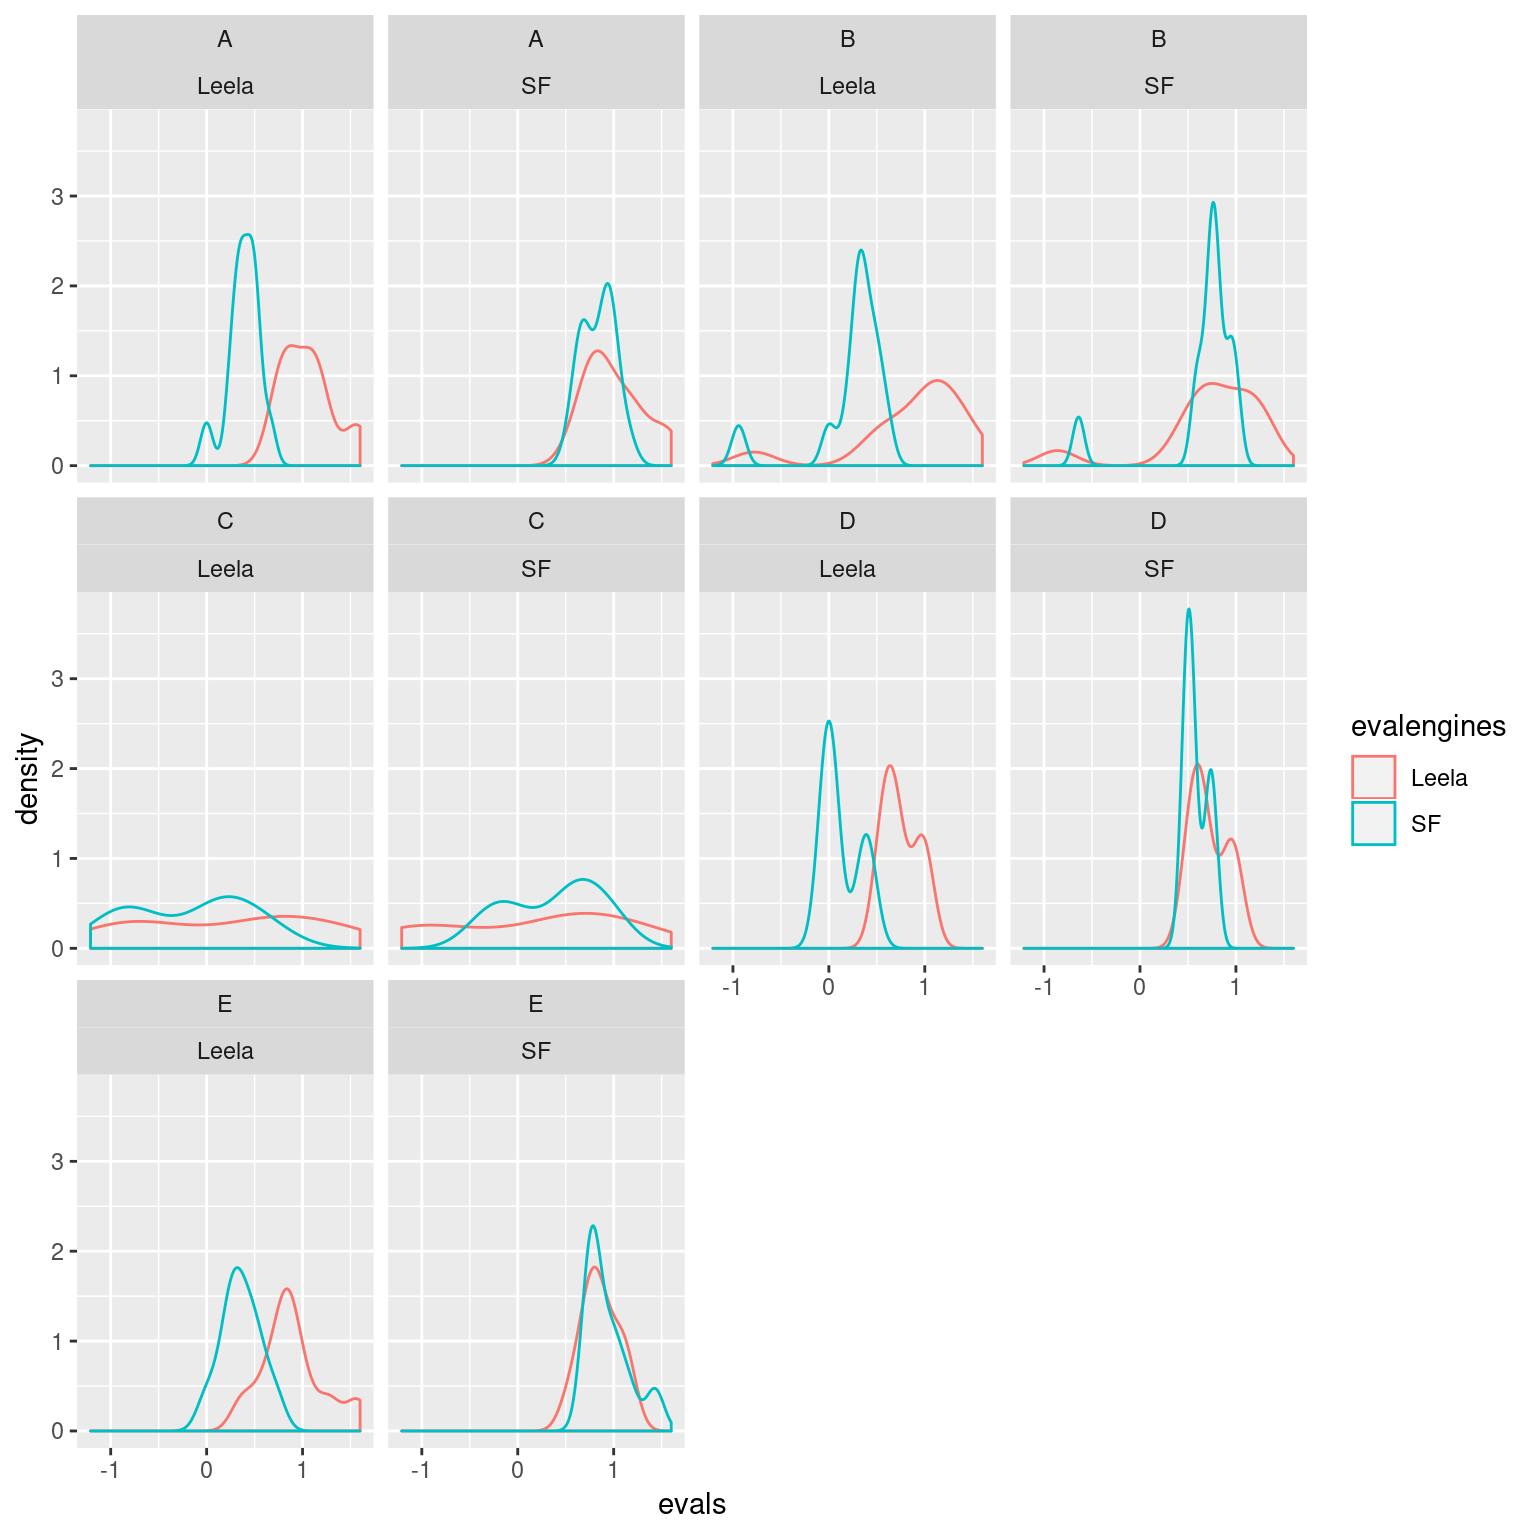
\includegraphics[width=3.14in,height=3.16in,keepaspectratio]{2018-05-28_elo_compute_files/figure-latex/unnamed-chunk-11-1.png}

\begin{Shaded}
\begin{Highlighting}[]
\NormalTok{data_df }\OperatorTok
\StringTok{  }\KeywordTok{filter}\NormalTok{(color }\OperatorTok{==}\StringTok{ "White"}\NormalTok{) }\OperatorTok
\StringTok{  }\KeywordTok{group_by}\NormalTok{(engine) }\OperatorTok
\StringTok{  }\KeywordTok{gather}\NormalTok{(evalengines, evals, Leela.openeval}\OperatorTok{:}\NormalTok{SF.openeval) }\OperatorTok
\StringTok{  }\KeywordTok{mutate}\NormalTok{(}\DataTypeTok{evalengines =} \KeywordTok{str_remove}\NormalTok{(evalengines, }\StringTok{".openeval"}\NormalTok{)) }\OperatorTok
\StringTok{  }\KeywordTok{ggplot}\NormalTok{(}\KeywordTok{aes}\NormalTok{(evals, }\DataTypeTok{color =}\NormalTok{ evalengines)) }\OperatorTok{+}\StringTok{ }
\StringTok{  }\KeywordTok{geom_density}\NormalTok{() }\OperatorTok{+}
\StringTok{  }\KeywordTok{facet_wrap}\NormalTok{(}\OperatorTok{~}\NormalTok{ECO2}\OperatorTok{+}\NormalTok{engine)}
\end{Highlighting}
\end{Shaded}

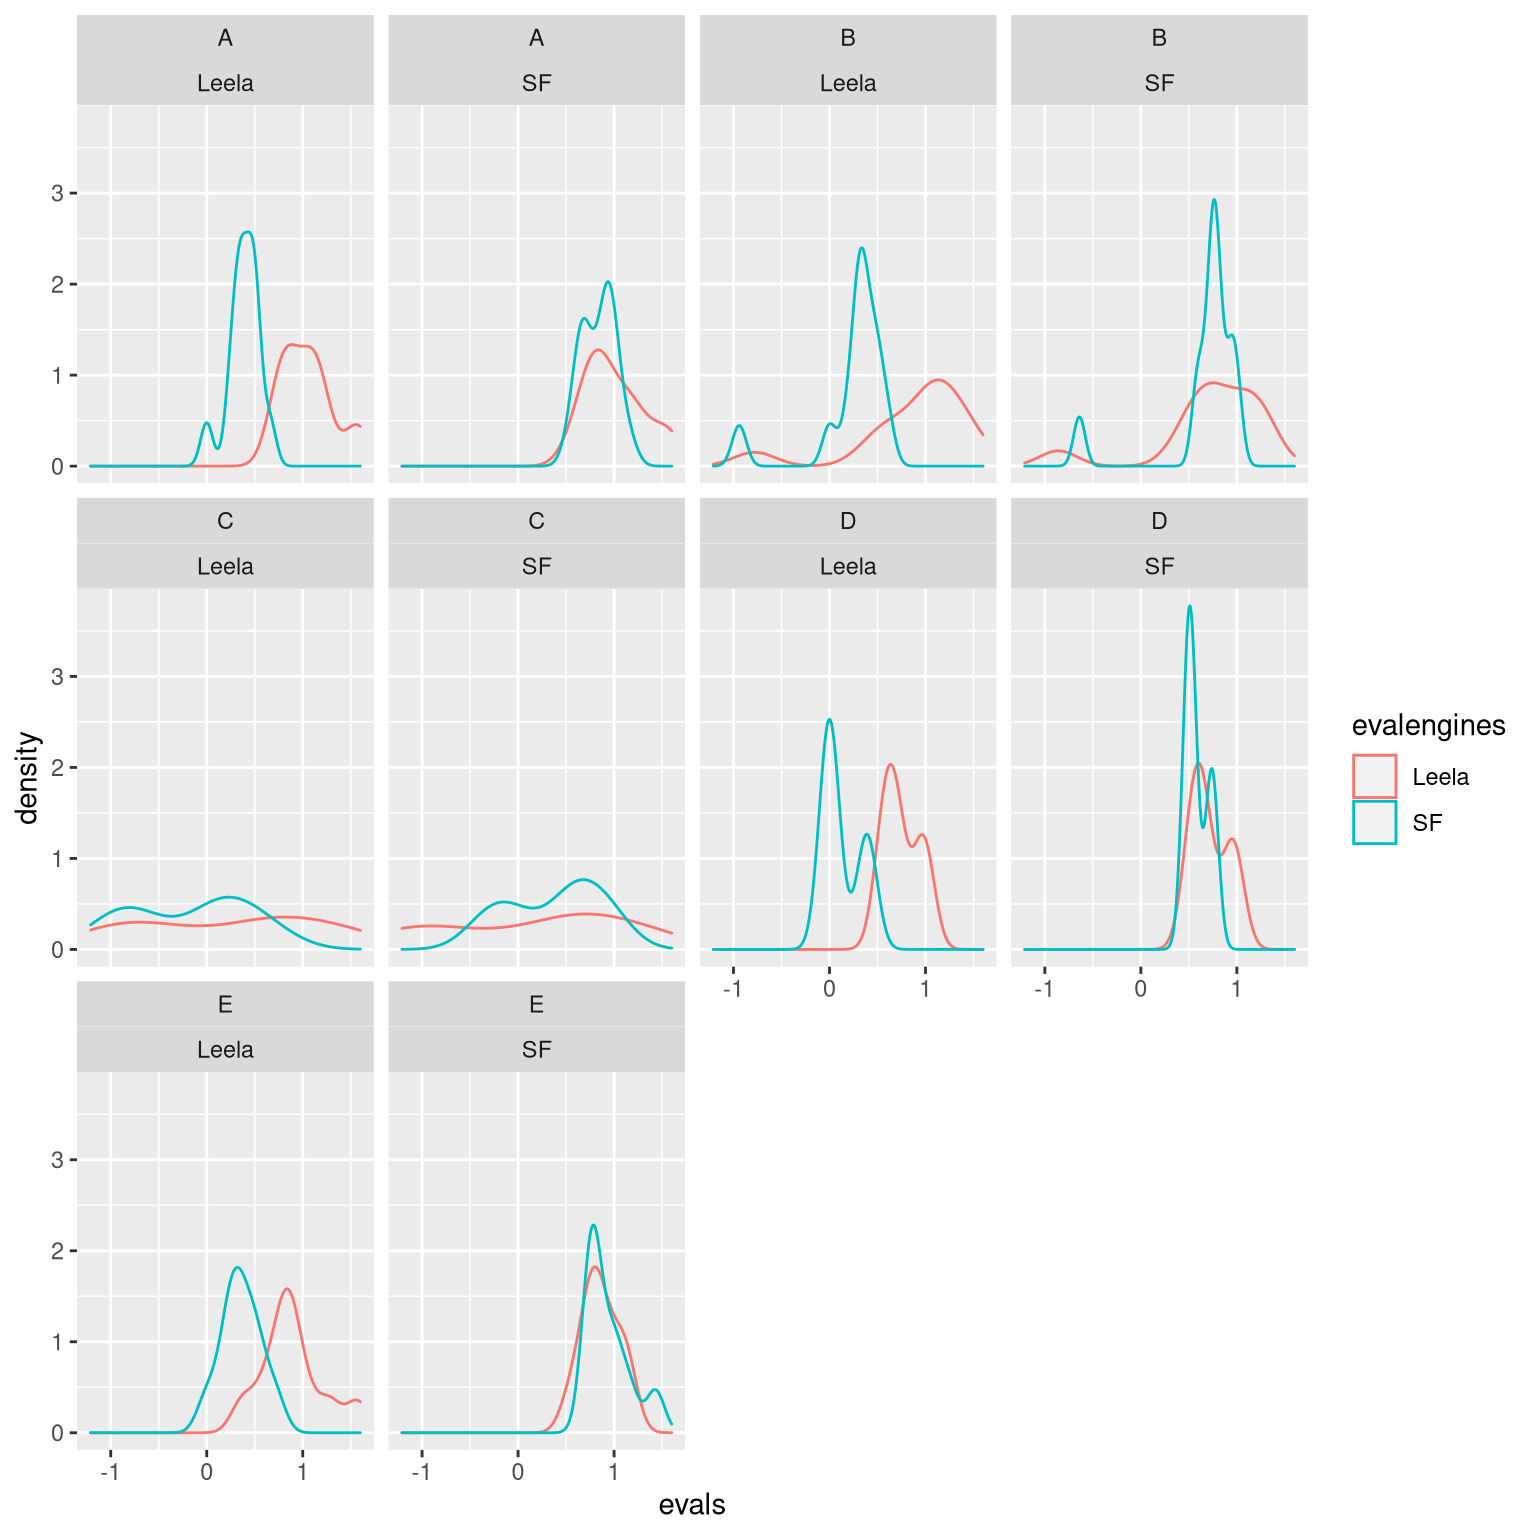
\includegraphics{2018-05-28_elo_compute_files/figure-latex/unnamed-chunk-12-1.pdf}

\begin{Shaded}
\begin{Highlighting}[]
\NormalTok{data_dfblack <-}\StringTok{ }\NormalTok{data_df }\OperatorTok
\StringTok{  }\KeywordTok{filter}\NormalTok{(color }\OperatorTok{==}\StringTok{ "Black"}\NormalTok{) }\OperatorTok
\StringTok{  }\KeywordTok{group_by}\NormalTok{(engine) }\OperatorTok
\StringTok{  }\KeywordTok{gather}\NormalTok{(evalengines, evals, Leela.openeval}\OperatorTok{:}\NormalTok{SF.openeval) }\OperatorTok
\StringTok{  }\KeywordTok{mutate}\NormalTok{(}\DataTypeTok{evalengines =} \KeywordTok{str_remove}\NormalTok{(evalengines, }\StringTok{".openeval"}\NormalTok{)) }\OperatorTok
\StringTok{  }\KeywordTok{group_by}\NormalTok{(ECO2, evalengines) }\OperatorTok
\StringTok{  }\KeywordTok{summarize}\NormalTok{(}\DataTypeTok{mean =} \KeywordTok{round}\NormalTok{(}\KeywordTok{mean}\NormalTok{(evals),}\DecValTok{3}\NormalTok{), }\DataTypeTok{sd =} \KeywordTok{round}\NormalTok{(}\KeywordTok{sd}\NormalTok{(evals),}\DecValTok{3}\NormalTok{))}
\NormalTok{data_dfblack }\OperatorTok\StringTok{ }\KeywordTok{flextable}\NormalTok{() }\OperatorTok\StringTok{ }\KeywordTok{autofit}\NormalTok{()}
\end{Highlighting}
\end{Shaded}

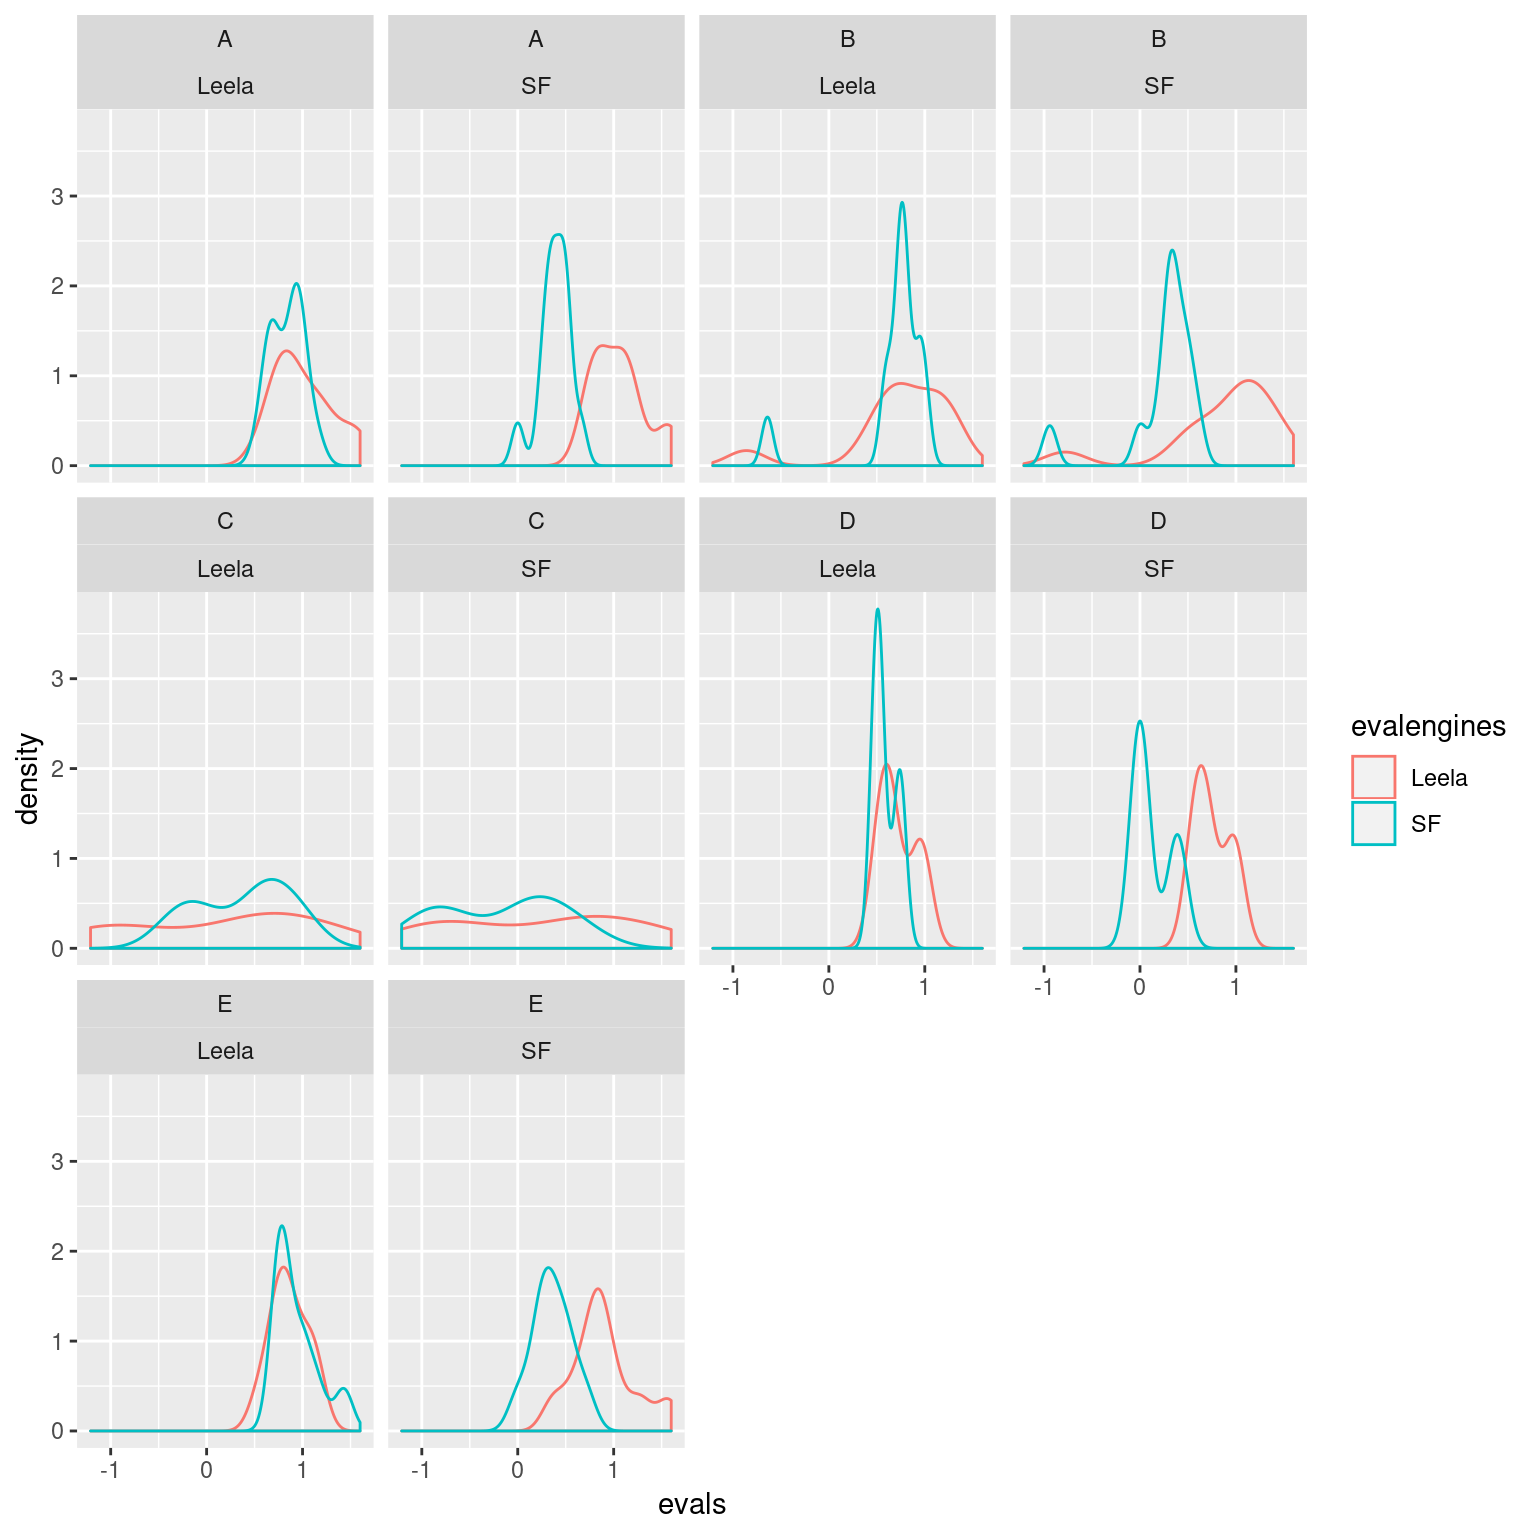
\includegraphics[width=3.14in,height=3.16in,keepaspectratio]{2018-05-28_elo_compute_files/figure-latex/unnamed-chunk-13-1.png}

\begin{Shaded}
\begin{Highlighting}[]
\NormalTok{data_df }\OperatorTok
\StringTok{  }\KeywordTok{filter}\NormalTok{(color }\OperatorTok{==}\StringTok{ "Black"}\NormalTok{) }\OperatorTok
\StringTok{  }\KeywordTok{group_by}\NormalTok{(engine) }\OperatorTok
\StringTok{  }\KeywordTok{gather}\NormalTok{(evalengines, evals, Leela.openeval}\OperatorTok{:}\NormalTok{SF.openeval) }\OperatorTok
\StringTok{  }\KeywordTok{mutate}\NormalTok{(}\DataTypeTok{evalengines =} \KeywordTok{str_remove}\NormalTok{(evalengines, }\StringTok{".openeval"}\NormalTok{)) }\OperatorTok
\StringTok{  }\KeywordTok{ggplot}\NormalTok{(}\KeywordTok{aes}\NormalTok{(evals, }\DataTypeTok{color =}\NormalTok{ evalengines)) }\OperatorTok{+}\StringTok{ }
\StringTok{  }\KeywordTok{geom_density}\NormalTok{() }\OperatorTok{+}
\StringTok{  }\KeywordTok{facet_wrap}\NormalTok{(}\OperatorTok{~}\NormalTok{ECO2}\OperatorTok{+}\NormalTok{engine)}
\end{Highlighting}
\end{Shaded}

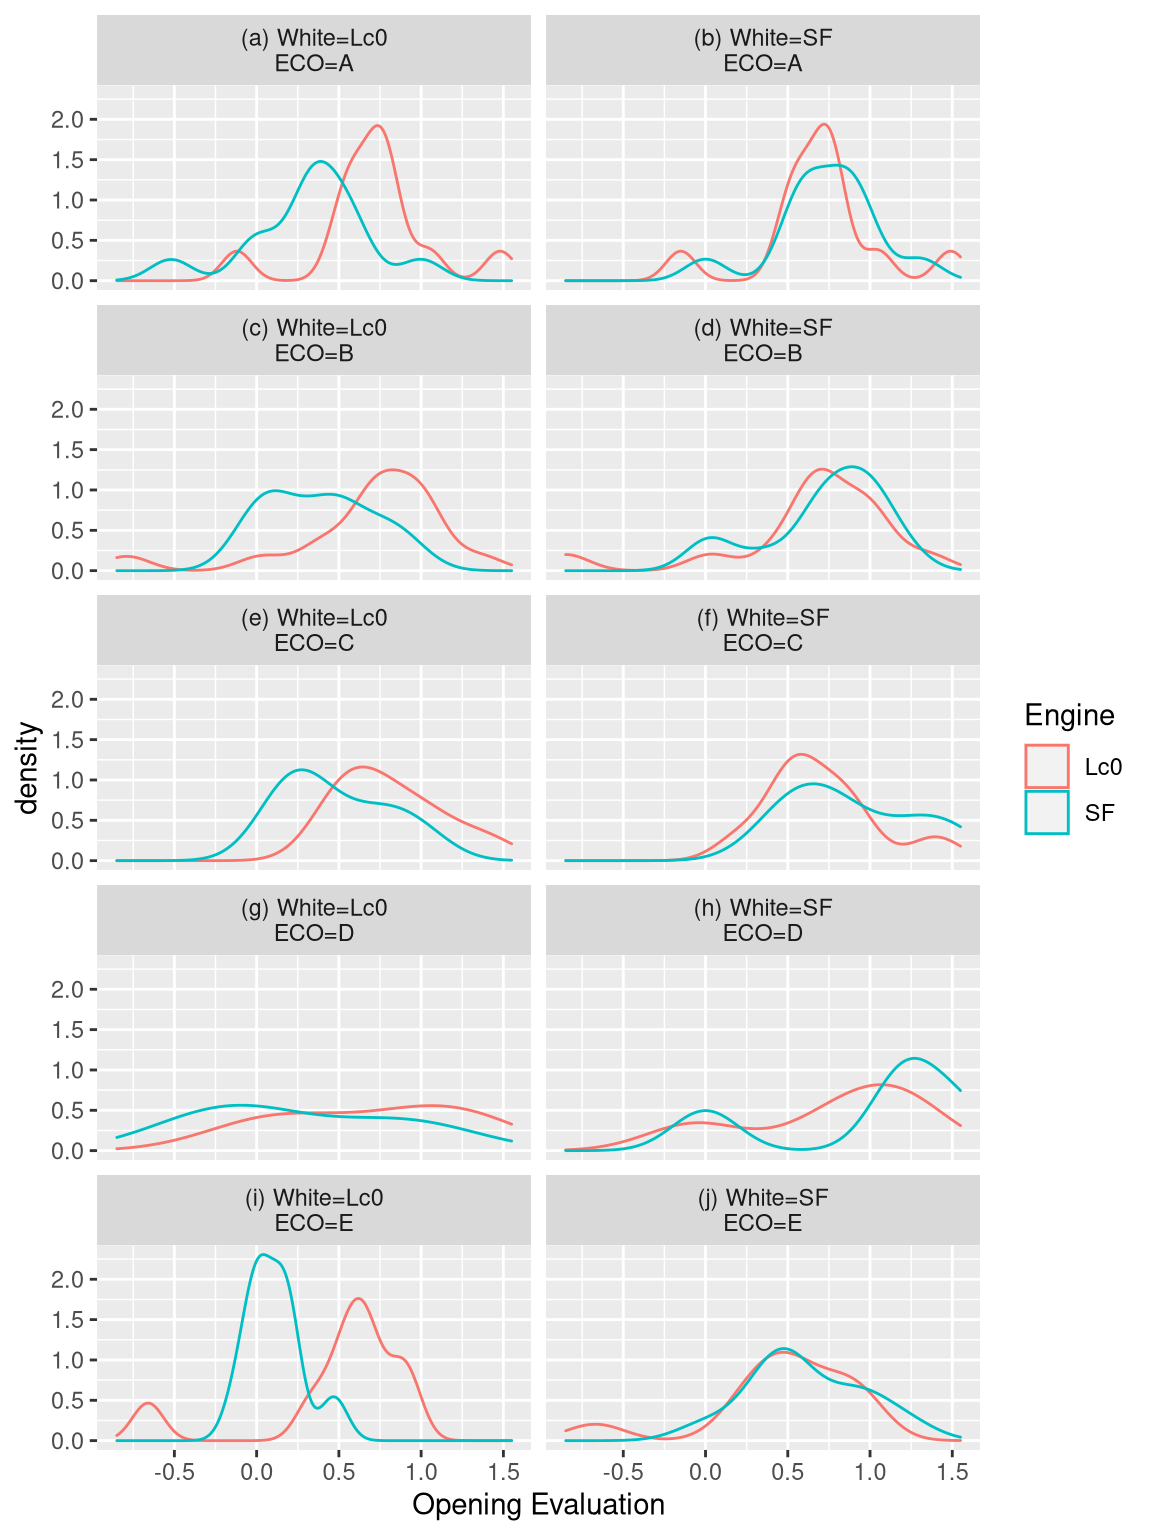
\includegraphics{2018-05-28_elo_compute_files/figure-latex/unnamed-chunk-14-1.pdf}

We can see that Leela's opening evals are generally more optimistic than
that of Stockfish, which can be attributed partly to SF's contempt. But
a closer inspection of Leela's evals, we see that they are consistent
even if playing as different colors. Leela also tends to win in openings
where its opening evals are visibly more optimistic than that of
Stockfish, signifying that Leela has better opening evaluation.

This has been a very exciting SuFi. I had a lot of fun engaging in many
interesting and lively discussions in chat, although oftentimes the chat
can quickly turn cancerous.

To end this post, I would like to congratulate the Leela devs and
community for winning their first ever SuFi title. Kudos also to the SF
team for continuing to improve a chess monster. I hope that Leela and SF
continue to expose each other's weaknesses, and get better as a result.
Exciting times for the chess engine fans!


\end{document}
